\documentclass[10pt]{article}
\usepackage{setup}
\usepackage[framed,numbered,autolinebreaks,useliterate]{mcode}
\vspace{-8ex}
\date{}

\graphicspath{{../figs/}}

\begin{document}

\title{\textbf{\Large{\textsc{ECE446:} Sensory Communication}} \\ \Large{Digital Signal Processing Problem Set Report}\vspace{-0.3cm}}
\author{Pranshu Malik\\ \footnotesize{1004138916}\vspace{-3cm}}

\maketitle

\section{Manipulation of Signals in the Frequency Domain}
To construct the signal in the frequency domain, we need to know the Fourier transform of the signal under consideration. The signal we want to construct are phasors, which are fundamentally cosine signals, i.e. $\text{Re}(Ae^{jf(t,\phi)}) = A\cos(f(t,\phi)) = Ae^{jg(\phi)} = \Tilde{A}$ for some functions $f$ and $g$. The continuous-time continuous-frequency Fourier transform (CTFT) for such a cosine is given by $\mathcal{F}\{\cos(\Omega_0t)\} = \pi(\delta(\Omega - \Omega_0) + \delta(\Omega + \Omega_0))$. Now, to be able to use this transform on a computer, we have to use the discrete-time discrete-frequency form of the Fourier transform, known as Discrete Fourier transform (DFT), and the fundamental idea behind it is to sample the continuous-frequency discrete-time Fourier transform (DTFT) at at equal intervals of $\frac{2\pi}{N}$ over a period of $2\pi$, be it from $[-\pi, \pi)$ or $[0, 2\pi)$, where $N$ is the number of points in the sampled signal of interest. The DTFT is a frequency-normalized and repeating version of CTFT of the signal, i.e. $X(e^{j\omega}) = \frac{1}{T_s}\sum_{k=-\infty}^{\infty}X_c(j(\frac{\omega}{T_s} - \frac{2\pi k}{T_s}))$, where $T_s = \frac{1}{F_s}$ is the sampling interval, $\omega = \Omega T \text{ [rad]}$ is the normalized angular frequency, and $X_c(j\Omega)$ is the CTFT of $x(t)$. Therefore, the DFT components for $0\leq k < N$ can be written as $X[k] = X(e^{j(\frac{2\pi}{N})k}) = X(e^{j\omega})\rvert_{\omega = (\frac{2\pi}{N})k}$, and zero for $k$ everywhere else. In code, we have followed this procedure to construct the DFT $X[k]$ of the desired signal $x[n]$ consisting of two phasors at frequencies $440$Hz and $660$Hz and with a relative phase shift of $\frac{\pi}{2}$. Thus, the result in time domain, we already know, should be match $\hat{x}(t) = \cos(2\pi440t) - \sin(2\pi660t)$ sampled at $t = nT_s$, i.e. $\hat{x}[n] \coloneqq \hat{x}(nT_s)$. This has been verified and the frequency and time domain plots for $x[n]$ are shown in figure \ref{freq_domain_design_for_time_domain_signal}.

\begin{figure}[ht]
    \centering
    \begin{subfigure}[b]{0.48\textwidth}
        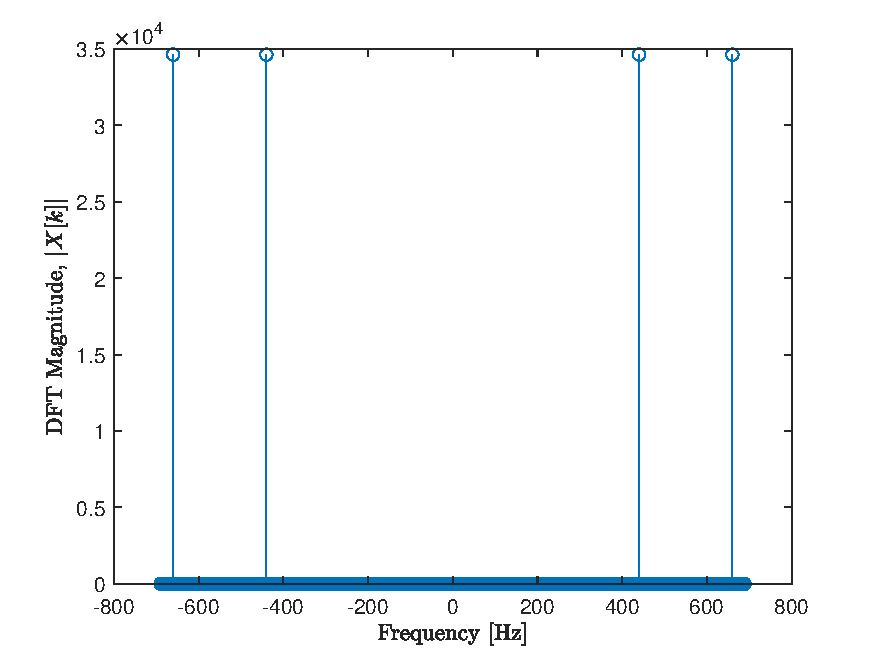
\includegraphics[width=\textwidth]{problem1_fft.pdf}
        % \caption{}
    \end{subfigure}
    \quad
    \begin{subfigure}[b]{0.48\textwidth}
        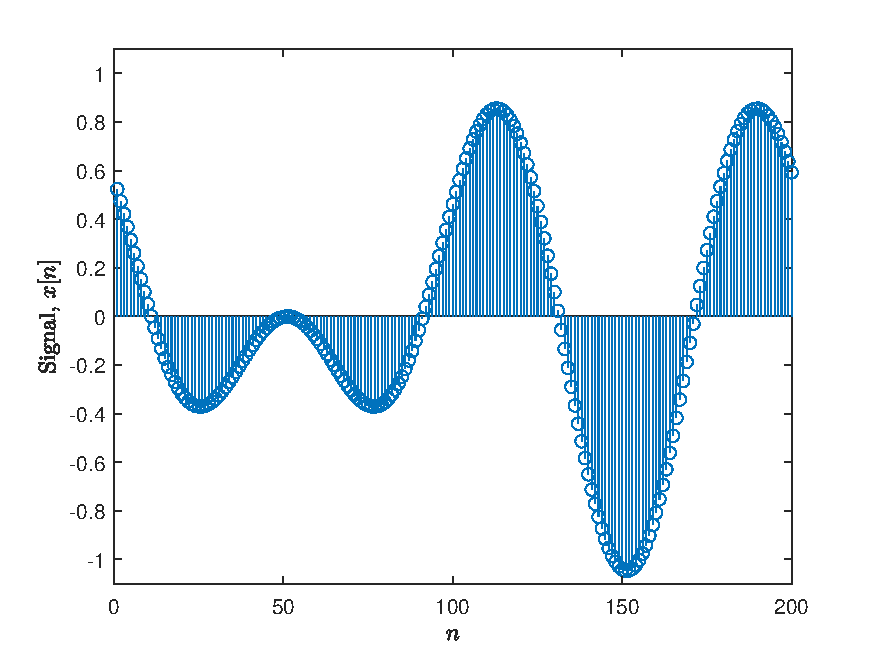
\includegraphics[width=\textwidth]{problem1_sig.pdf}
        % \caption{}
    \end{subfigure}
    \caption{Frequency and time domain representations of $x[n]$\vspace{-0.5cm}}
    \label{freq_domain_design_for_time_domain_signal}
\end{figure}

\section{Effect of Time Windowing on the Frequency Spectra}

We can practically only observe finite length signals, and this has a fundamental implication on how well we can localize the frequency information over the time which it happens. This is known as the time-frequency trade-off, which arises due to the convolution of the time-window spectra with the spectra of the infinite-length signal. Figures \ref{time_bandwidth_tradeoff} (a) and (b) show the effect of relatively decreasing the observation time window of a sinusoidal signal, where we can clearly see that in (a) the energy is more sharply localized at frequency $f_0 = 1000$Hz while (b) has larger spread (or distortion) around $f_0$ with a broader $\text{sinc}$ function. As a limiting case, we would expect the positive spectra to converge to a $\delta$ function for an infinite-length time window. In general, this is expressed as the time-bandwidth relation where $\Delta f$ is the observed bandwidth and $\Delta t$ is the observation period,

\[
\Delta f \Delta t \geq 1 
\]

\begin{figure}[ht]
    \centering
    \begin{subfigure}[b]{0.48\textwidth}
        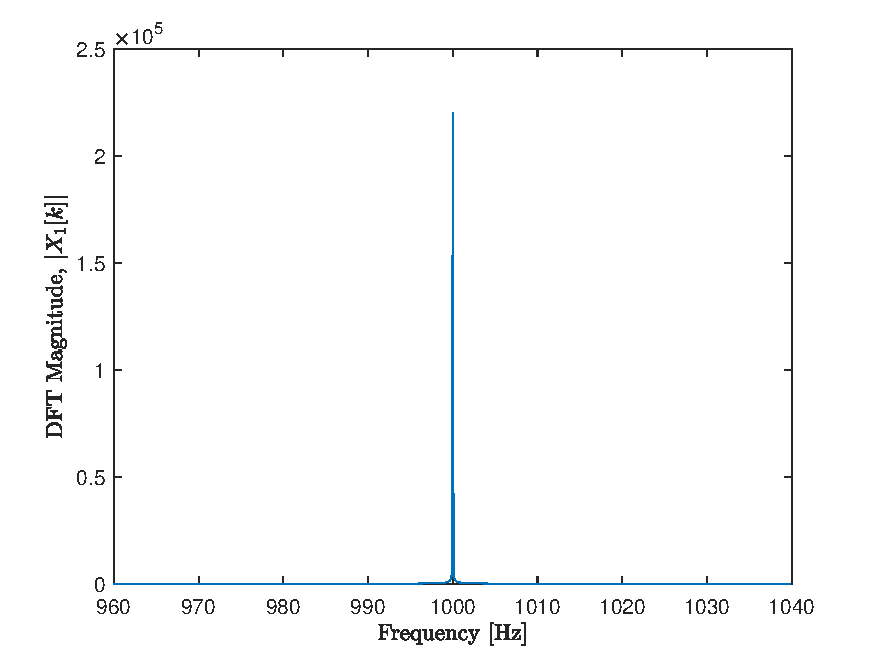
\includegraphics[width=\textwidth]{problem2_fft_high_dur.pdf}
        \caption{Spectra for $\Delta t=10$s}
    \end{subfigure}
    \quad
    \begin{subfigure}[b]{0.48\textwidth}
        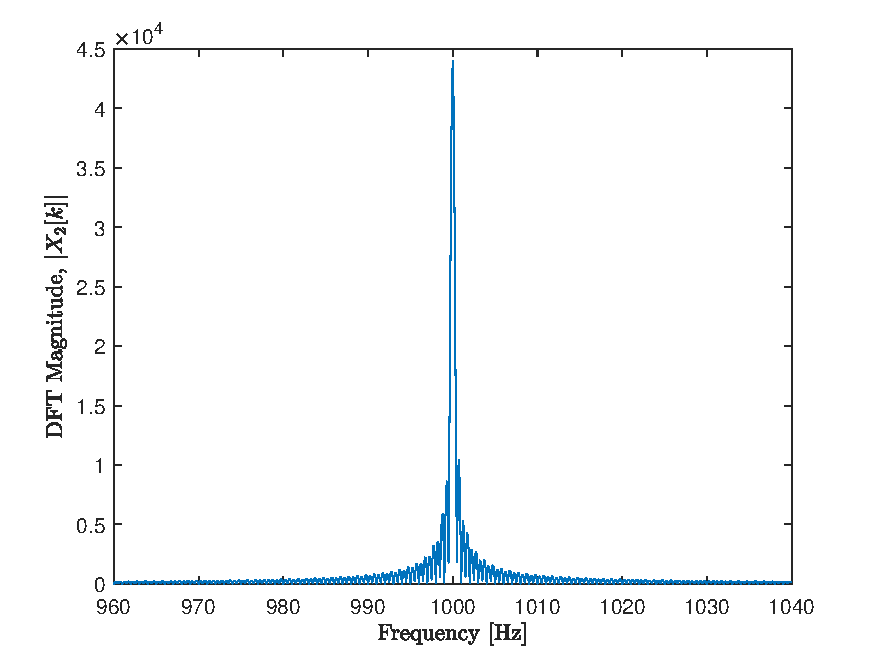
\includegraphics[width=\textwidth]{problem2_fft_low_dur.pdf}
        \caption{Spectra for (net) $\Delta t=2$s}
    \end{subfigure}
    \caption{Effect of decreasing time window on frequency spectra\vspace{-0.5cm}}
    \label{time_bandwidth_tradeoff}
\end{figure}

\section{Telephone Dial Tones}
Each dial tone signal was generated adding two sinusoidal signals with the corresponding frequencies $f_\text{lower}$ and $f_\text{upper}$ listed in the DTMF (dual-tone multi-frequency) standard table.
\[
    \frac{1}{2}(\cos(2\pi f_\text{lower}t) + \cos(2\pi f_\text{upper}t))
\]

\section{Dial Tone Decode Algorithm}
Given a DTMF signal, we would like to decode which key it corresponds to. This can be easily achieved once we know the $f_\text{lower}$ and $f_\text{upper}$ frequencies involved in the signal. Although this can be done using an analog circuit with tuned filters (in parallel) with a mediocre $Q$ for making them robust to noise on the channel, we would like to develop the digital version of the process, an algorithm, that can be implemented, for example, on a microprocessor. Moreover, to  make it robust to noise and distortion in the same way as the circuits, we introduce an $\epsilon -$frequency band around each DTMF frequency bin. The procedure for this is listed in algorithm \ref{alg:dtmf_decode_algorithm}, and the corresponding \textsc{MATLAB} code can be found in the appendix.

\begin{figure}[ht]
  \centering
  \begin{minipage}{.64\linewidth}
        \begin{algorithm}[H]
            \caption{Robust DTMF Decoder}
            \label{alg:dtmf_decode_algorithm}
            \begin{algorithmic}
                \Require Signal $x[n]$, sampling rate $F_s$, DTMF table $(L, U) \mapsto k$
                \State $\epsilon \gets \texttt{fr\_eps}$
                \State $X \gets \mathcal{F}\{x[n]\}$ \Comment{FFT of the signal}
                \For{$\forall f_{l,i} \in f_\text{lower} \text{ and } \forall f_{u,j} \in f_\text{upper}$}
                    \State $m_{l, i} \gets \sum_f||X(f-f_{l,i} < \epsilon)||$
                    \State $m_{u, j} \gets \sum_f||X(f-f_{u,j} < \epsilon)||$
                \EndFor
                \State $L = \argmax_i \quad [m_{l, i}]$  \Comment{Get index of the maximum}
                \State $U = \argmax_j \quad [m_{u, j}]$
                \State \Return DTMF$(L, U)$ \Comment{corresponding key $k$ is returned}
            \end{algorithmic}
        \end{algorithm}
    \end{minipage}
    \caption{Algorithm for decoding DTMF tones to the corresponding key}
\end{figure}

\section{Telephone Event Tones}
The tones for busy and continuous dial events were generated using the method described in section 3.

\section{Helmholtz Resonators}
The Helmholtz frequency for a resonator, $\omega_H = 2\pi f_H$, is given by $\omega_H = c\sqrt{\frac{S}{V_0l}}$, where $S$ is the cross-sectional area of the neck, $l$ is the length of the neck, $V_0$ is the volume of the cavity or resonator, and $c=343$m/s is the speed of sound at $20^\circ$C. For a chosen bottle as a Helmholtz resonator, we were interested in finding its resonant frequency and its change with a decrease in available volume by a factor. After repeated trials, this factor was chosen to be $\frac{1}{3}$ instead of the suggested value of $\frac{1}{2}$, mainly since it was harder to achieve resonance for the half-filled bottle without creating excess noise caused by the blowing of air. Due to the volume change, we then had the cavity volume $V_1 = \frac{2}{3}V_0$ and we expected the observed resonant frequencies to shift by a factor of $\frac{\widehat{\omega_H}}{\omega_H} = \sqrt{\frac{V_0}{V_1}} = \sqrt{\frac{3}{2}}$. The chosen bottle had $V_0 = 750$ml, $l=1$cm, and cross-sectional diameter $D=2$cm. The resonant frequencies were observed as peaks on the FFT spectra shown in figure \ref{helmholtz_resonance}. For the empty bottle, we observed $f_h = 153.4$Hz, which is different from the expected value of $f_{H, \text{exp}} = 353.3$Hz. This could be because of the larger mouth of the bottle and the assumption for $V_0 \gg Sl$ not holding that well. However, the expected resonant frequency, $f_{H, \text{exp}} = 158$Hz, comes closer to $f_{H}$ for $l=5$cm. The observed frequency for the one-third filled bottle was $\widehat{f_H} = 190.7$Hz which is close to $f_H\sqrt{\frac{3}{2}} = 187.87\text{Hz} \approx 190.7$Hz. This confirms the inverse $\sqrt{V}$ relationship with the resonant frequency even if the apparent parameters for the resonator might be different than the measurements.

\begin{figure}[ht]
    \centering
    \begin{subfigure}[b]{0.48\textwidth}
        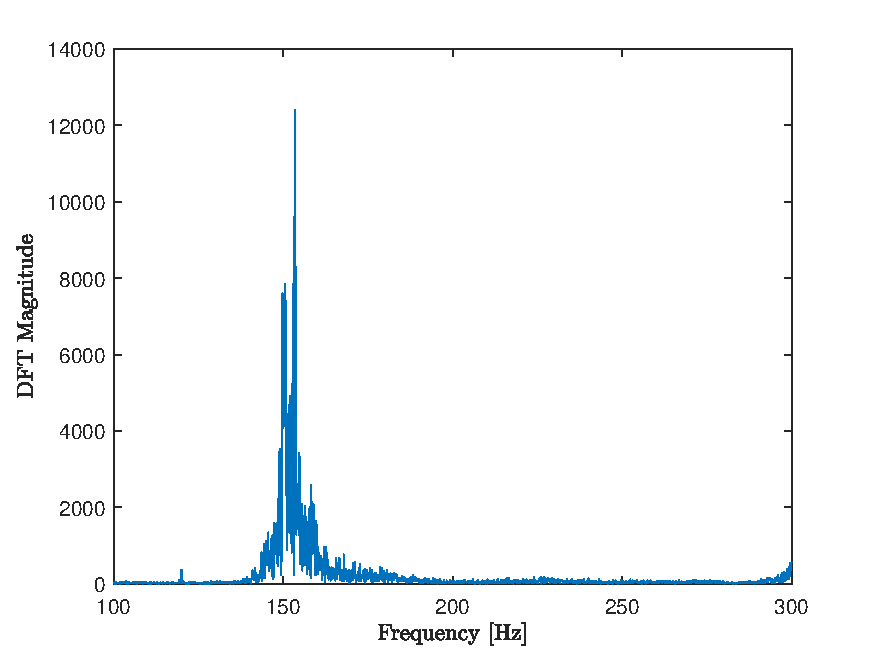
\includegraphics[width=\textwidth]{problem6_empty_bottle_resonance_spectra.pdf}
        \caption{$f_H$ for empty bottle}
    \end{subfigure}
    \quad
    \begin{subfigure}[b]{0.48\textwidth}
        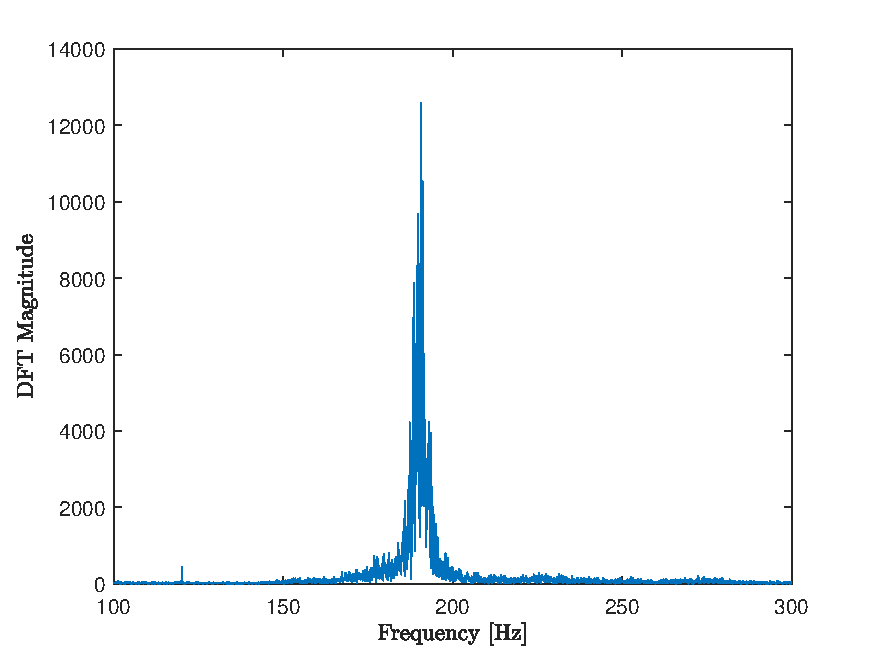
\includegraphics[width=\textwidth]{problem6_filled_bottle_resonance_spectra.pdf}
        \caption{$f_H$ for one-third filled bottle}
    \end{subfigure}
    \quad
    \begin{subfigure}[b]{0.48\textwidth}
        \centering
        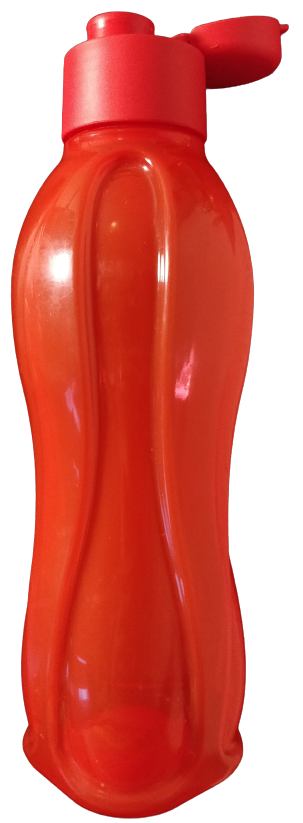
\includegraphics[scale=0.15]{bottle.png}
        \caption{Helmholtz resonator}
    \end{subfigure}
    \caption{Observing Helmholtz resonance in a bottle\vspace{-0.5cm}}
    \label{helmholtz_resonance}
\end{figure}

\section{Comparison of Voice and Instrument Timbre}
Violin has 440 as the fundamental harmonic and has 2 sub harmonics and all above; structure to the spread. Voice has two main harmonics 440 and 220 and they reduce in magnitude, without much "structure". Shows different timbre (or lack of, thereof). Notice the location of the peaks and the relative magnitudes of the peak. What do you see in common, what is different between the voice and the musical instrument?

\begin{figure}[ht]
    \centering
    \begin{subfigure}[b]{0.48\textwidth}
        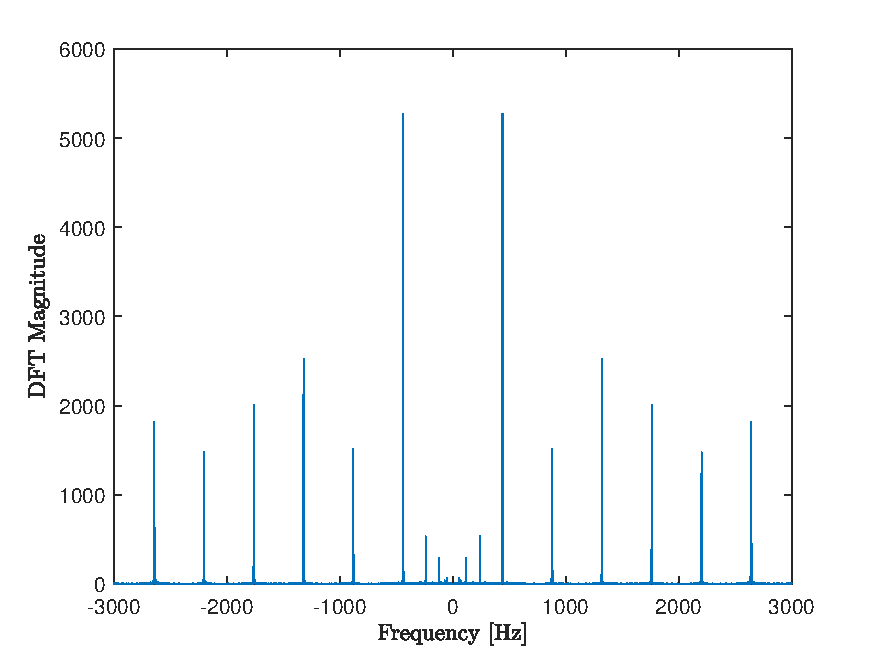
\includegraphics[width=\textwidth]{problem7_a440_violin_spectra.pdf}
        \caption{High Dur}
    \end{subfigure}
    \quad
    \begin{subfigure}[b]{0.48\textwidth}
        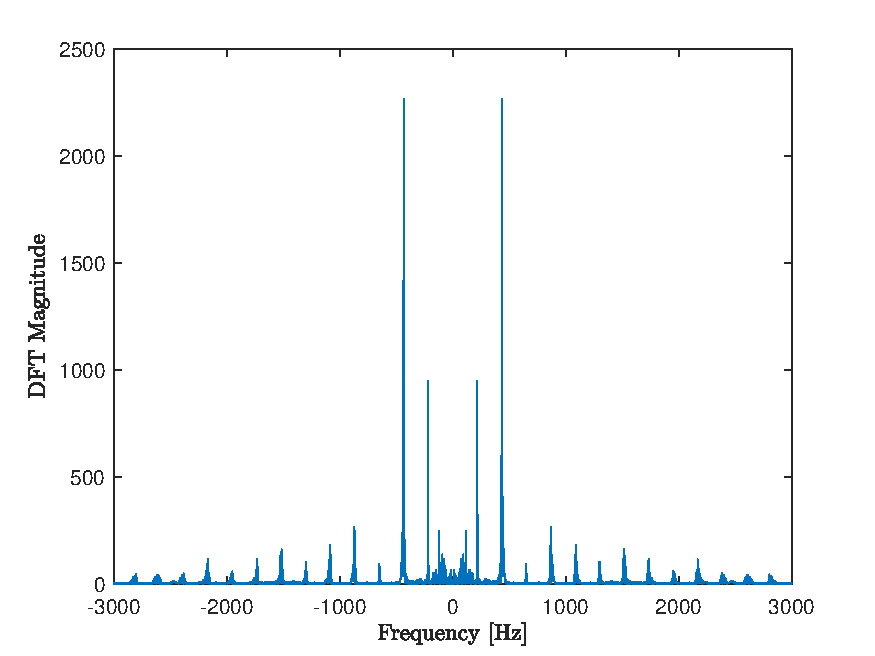
\includegraphics[width=\textwidth]{problem7_a440_voice_spectra.pdf}
        \caption{Low Dur}
    \end{subfigure}
    \quad
    \begin{subfigure}[b]{0.48\textwidth}
        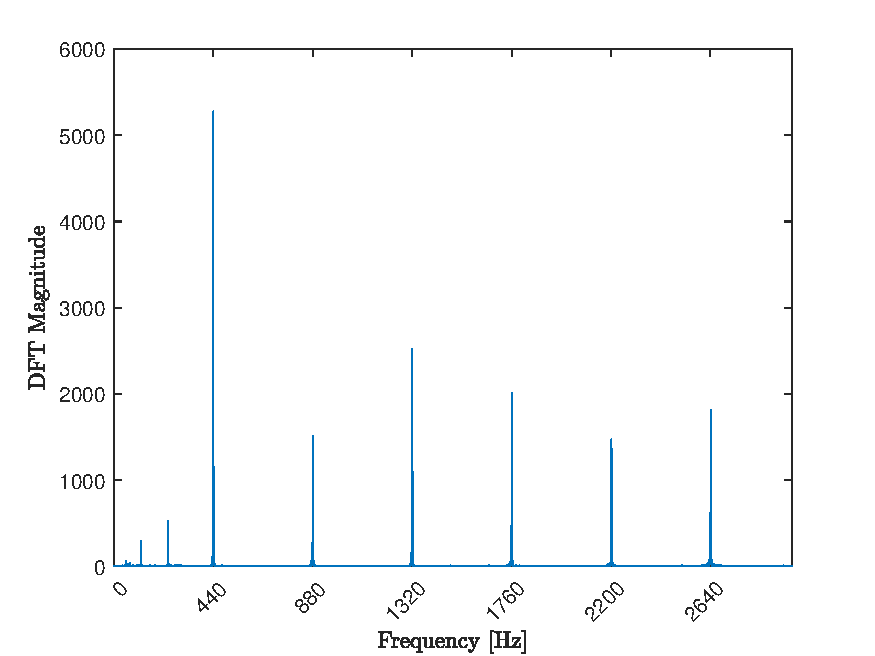
\includegraphics[width=\textwidth]{problem7_a440_violin_harmonics.pdf}
        \caption{Violin Harmonics}
    \end{subfigure}
    \quad
    \begin{subfigure}[b]{0.48\textwidth}
        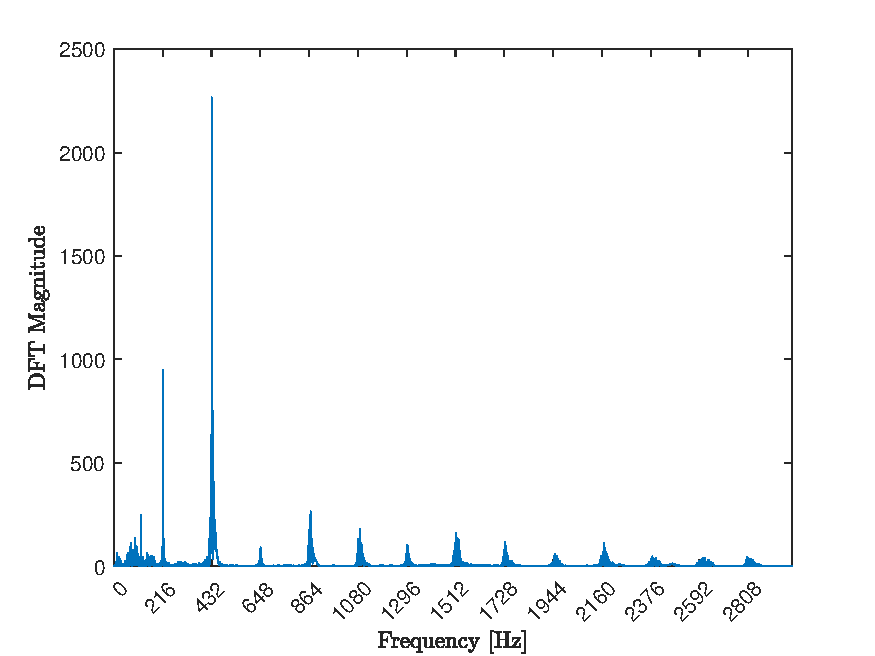
\includegraphics[width=\textwidth]{problem7_a440_voice_harmonics.pdf}
        \caption{Low Dur}
    \end{subfigure}
    % \quad
    % \begin{subfigure}[b]{0.48\textwidth}
    %     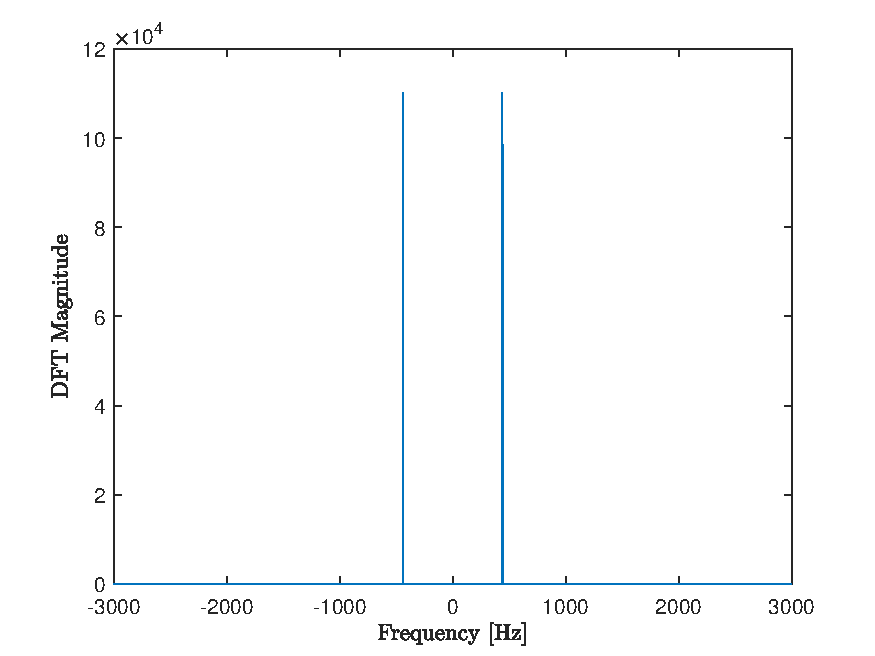
\includegraphics[width=\textwidth]{problem7_a440_pure_spectra.pdf}
    %     \caption{Low Dur}
    % \end{subfigure}
    \caption{Spectra and Harmonics of the Signals\vspace{-0.5cm}}
    \label{note_timbre_harmonics}
\end{figure}

Notice that the harmonics are present at multiple types and for diff frequencies.

\section{Creating Chirps}
Done.

\begin{figure}[ht]
    \centering
    \begin{subfigure}[b]{0.48\textwidth}
        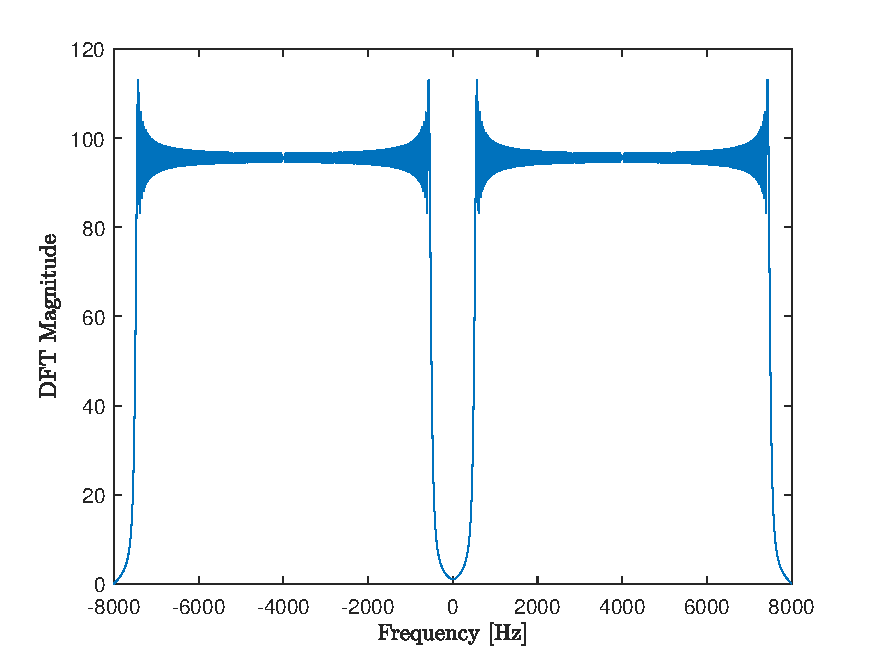
\includegraphics[width=\textwidth]{problem8_fft_linear_chirp.pdf}
        \caption{High Dur}
    \end{subfigure}
    \quad
    \begin{subfigure}[b]{0.48\textwidth}
        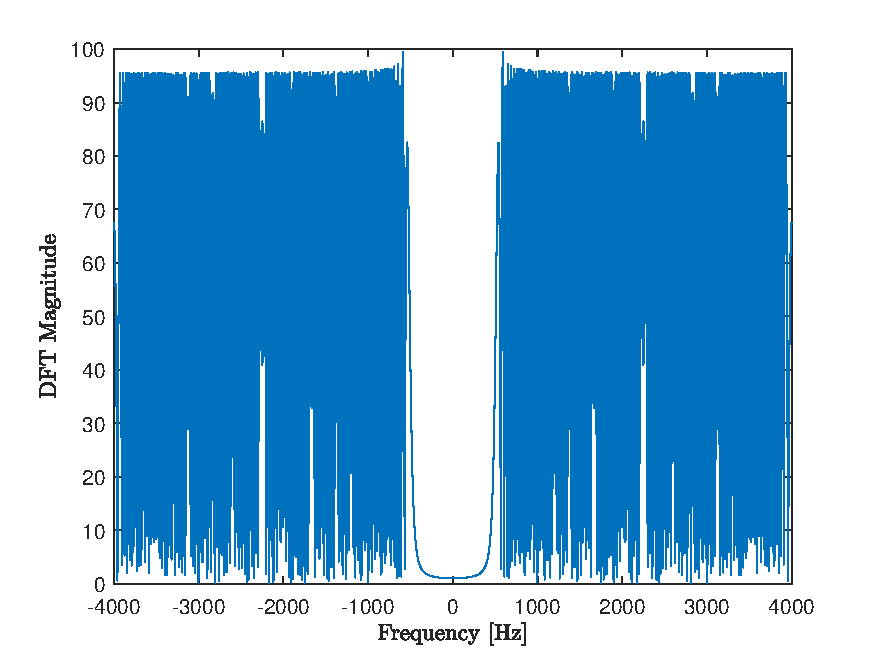
\includegraphics[width=\textwidth]{problem8_fft_subsampled_linear_chirp.pdf}
        \caption{Low Dur}
    \end{subfigure}
    \caption{Linear Chirps\vspace{-0.5cm}}
    \label{linear_chirp_fft}
\end{figure}

\section{Developing Simple Spectrograms}
Done. The spectrogram was made using rectangular windows with no overlaps. This causes spctral leakage, but since we have crafted a signal with exact frequencies and single tones at any given time, the spectrogram is very clear. Check figure xyz. In code, we call this manual construction function a \texttt{sonograph} as an alias, since the \texttt{spectrogram} function already exists in \textsc{MATLAB}.

\begin{figure}[ht]
    \centering
    \begin{subfigure}[b]{0.48\textwidth}
        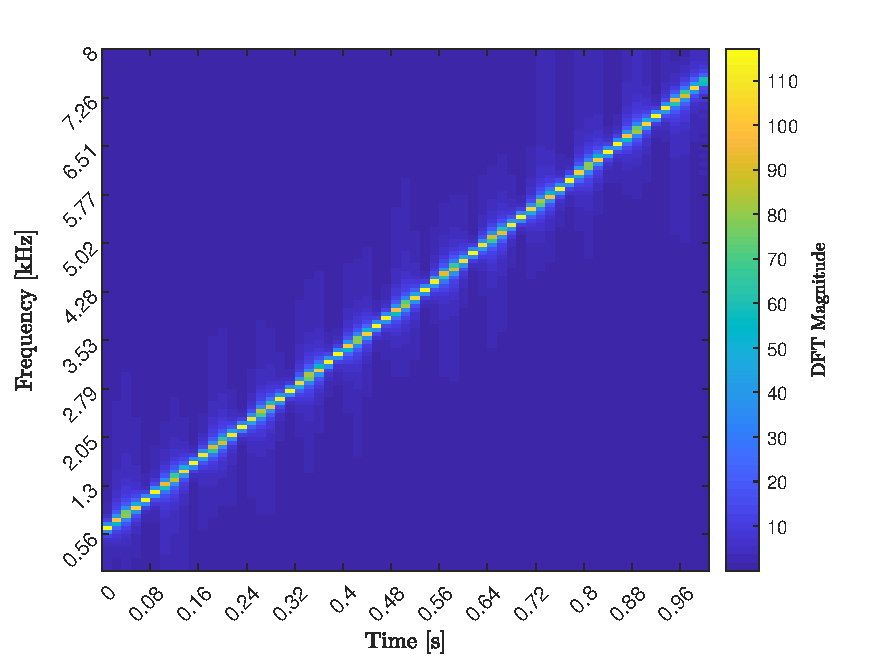
\includegraphics[width=\textwidth]{problem9_sonogram_linear_chirp.pdf}
        \caption{High Dur}
    \end{subfigure}
    \quad
    \begin{subfigure}[b]{0.48\textwidth}
        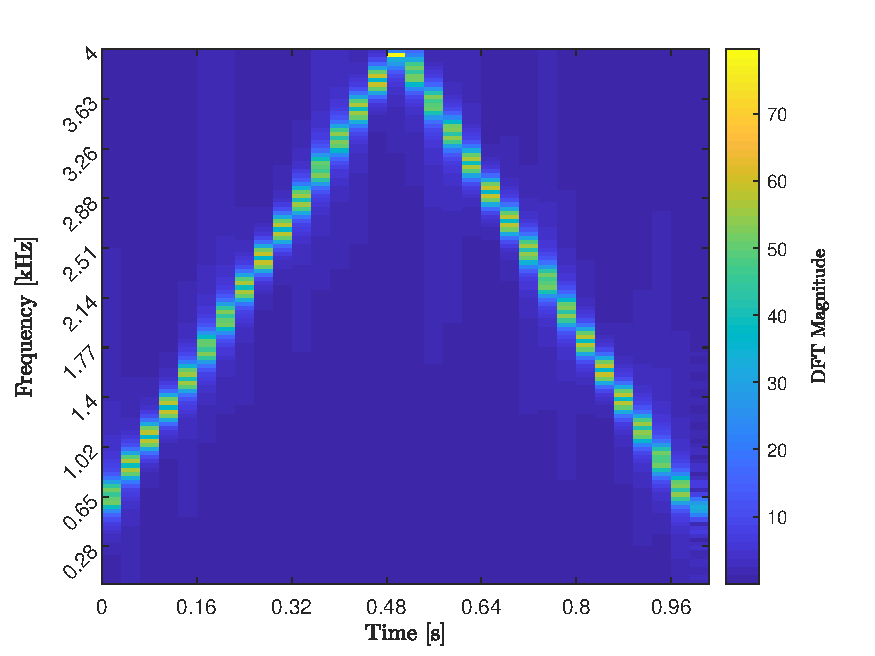
\includegraphics[width=\textwidth]{problem9_sonogram_subsampled_linear_chirp.pdf}
        \caption{Low Dur}
    \end{subfigure}
    \caption{Linear Chirps\vspace{-0.5cm}}
    \label{linear_chirp_spectrogram}
\end{figure}

\section{Doppler Effect and Tracking Chirps on Spectrograms}
The apparent frequency is:
\[
f_\text{app}(t) = f_0 \frac{c}{c + v\sin\left(\arctan\left(\frac{v(t-t_0)}{d}\right)\right)}
\]

Where it crosses the closest distance $d$ at $t = t_0$.

$f_0 = 6.7418e+03$, $v = 84.4658$, $d=40.4337$, $t_0 = 3.29$s.

\begin{figure}[ht]
    \centering
    \begin{subfigure}[b]{0.48\textwidth}
        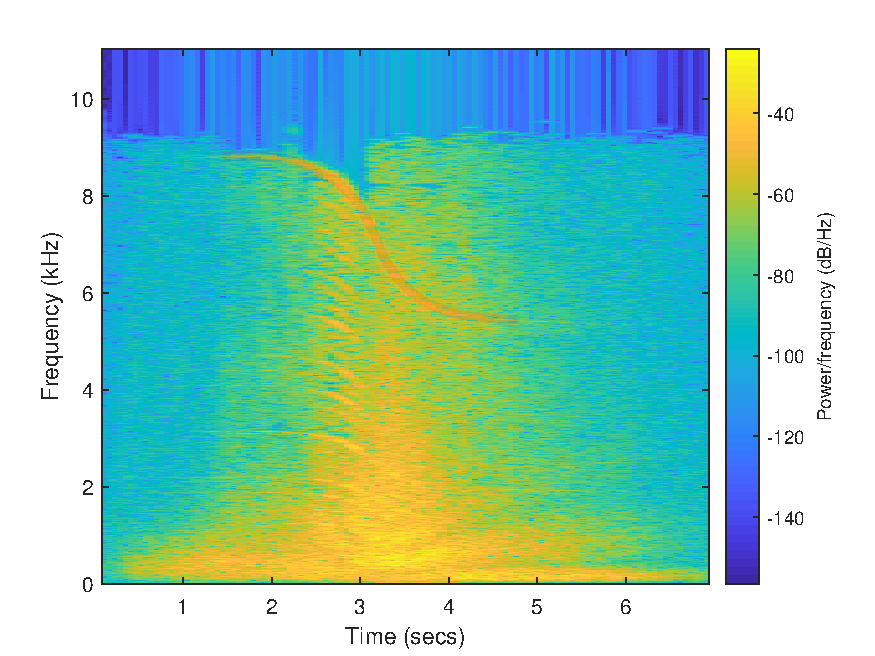
\includegraphics[width=\textwidth]{problem10_jet_spectrogram_doppler_shift_tracking.pdf}
        \caption{High Dur}
    \end{subfigure}
    \quad
    \begin{subfigure}[b]{0.48\textwidth}
        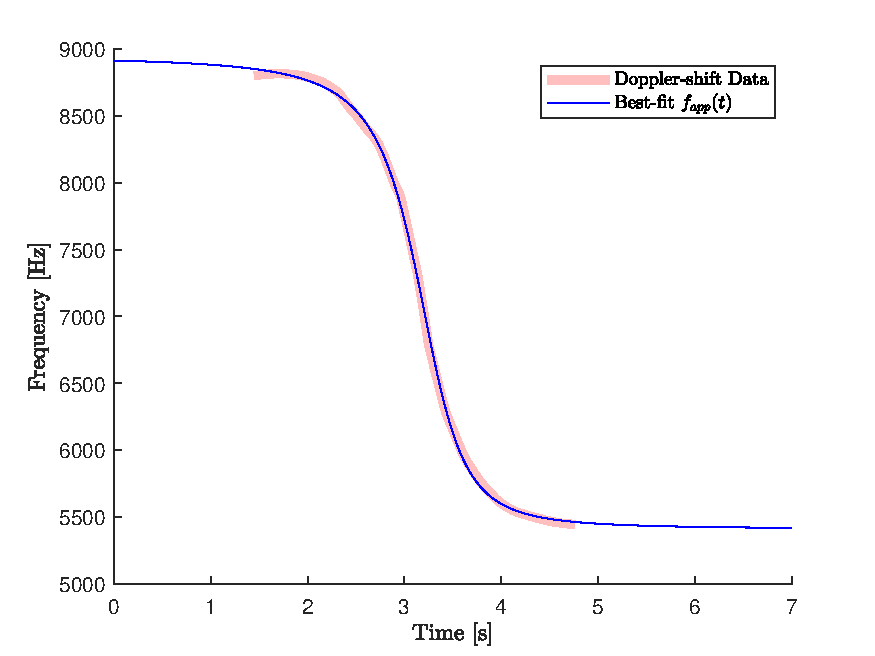
\includegraphics[width=\textwidth]{problem10_f_app_best_fit_estimate.pdf}
        \caption{Low Dur}
    \end{subfigure}
    \caption{Doppler Shift Tracking and Estimate\vspace{-0.5cm}}
    \label{doppler_shift_chirp}
\end{figure}

\section{Generating Random Noise}
Done. White: ; Pink: Low-frequency filtering of a white noise signal; Brown: Integration of a white noise signal. Give the procedure followed in code.

\begin{figure}[ht]
    \centering
    \begin{subfigure}[b]{0.31\textwidth}
        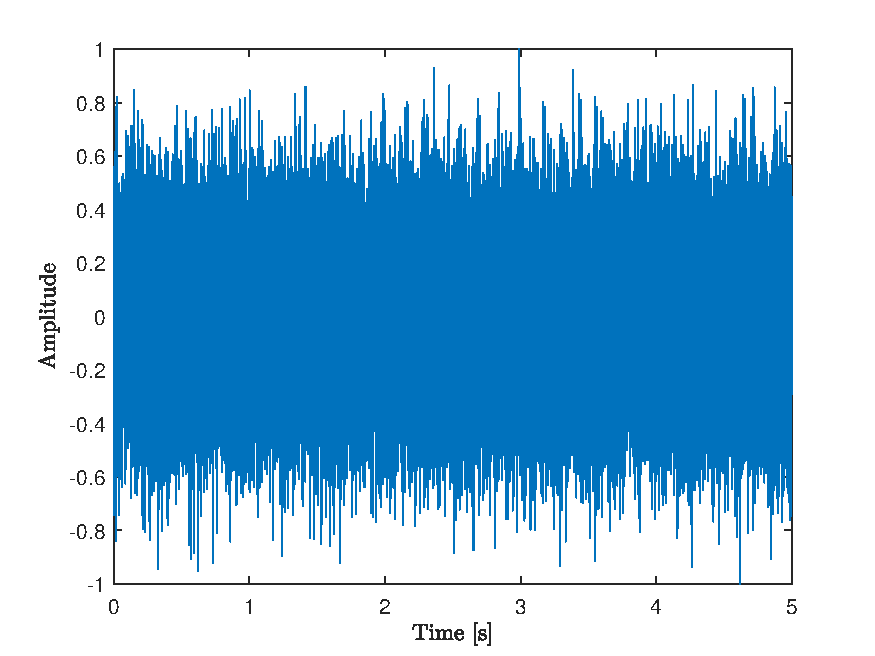
\includegraphics[width=\textwidth]{problem11_white_noise_time.pdf}
        \caption{High Dur}
    \end{subfigure}
    \quad
    \begin{subfigure}[b]{0.31\textwidth}
        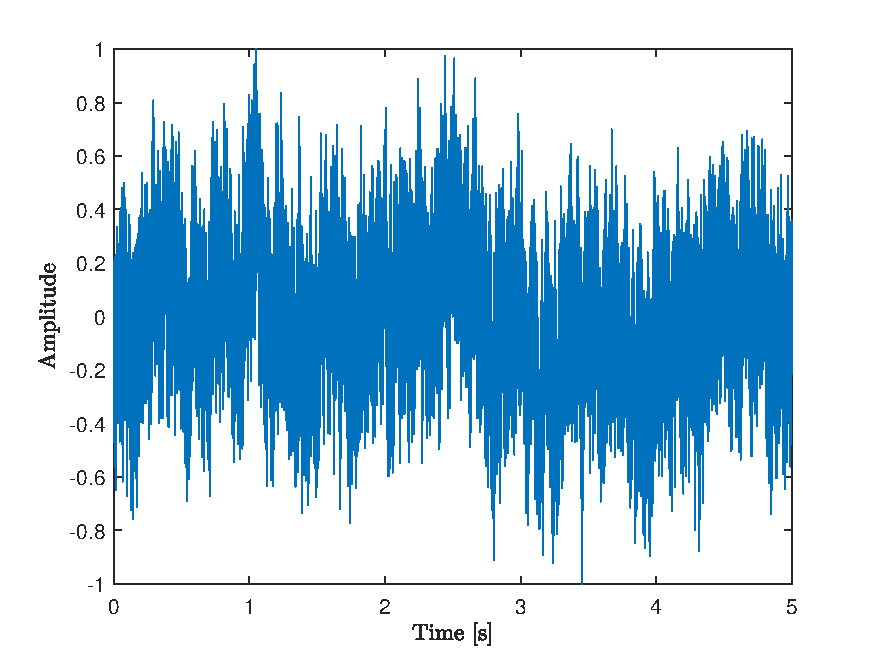
\includegraphics[width=\textwidth]{problem11_pink_noise_time.pdf}
        \caption{Low Dur}
    \end{subfigure}
    \quad
    \begin{subfigure}[b]{0.31\textwidth}
        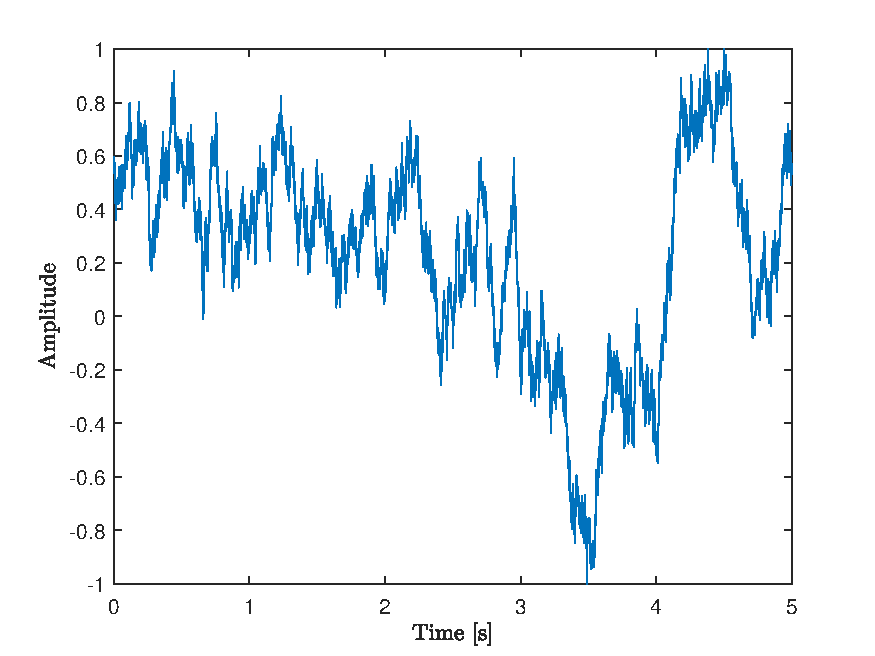
\includegraphics[width=\textwidth]{problem11_brown_noise_time.pdf}
        \caption{Low Dur}
    \end{subfigure}
    \caption{Color Noise in Time Domain\vspace{-0.5cm}}
    \label{color_noise_time_domain}
\end{figure}

\begin{figure}[ht]
    \centering
    \begin{subfigure}[b]{0.31\textwidth}
        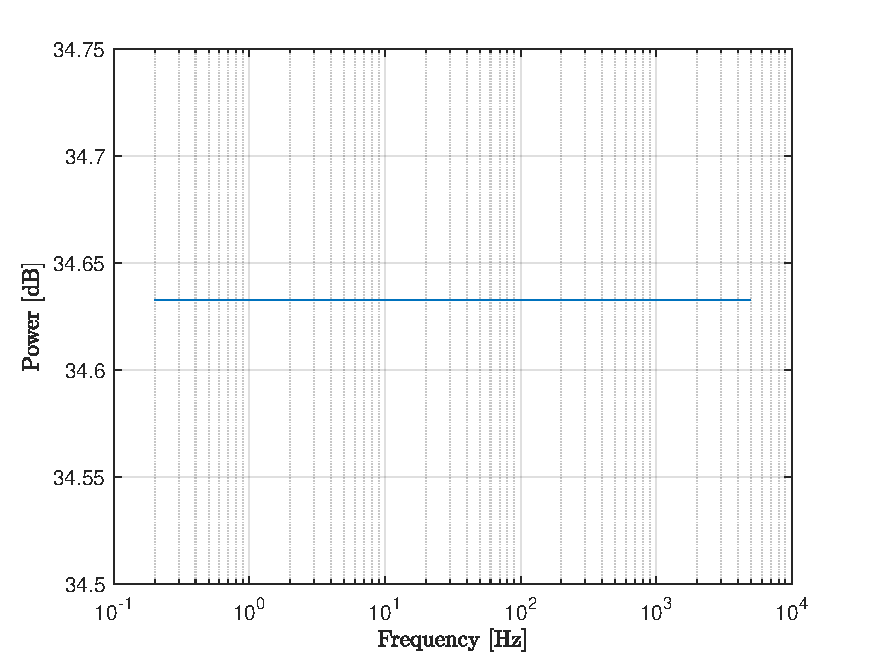
\includegraphics[width=\textwidth]{problem11_white_noise_power_spectrum_db.pdf}
        \caption{High Dur}
    \end{subfigure}
    \quad
    \begin{subfigure}[b]{0.31\textwidth}
        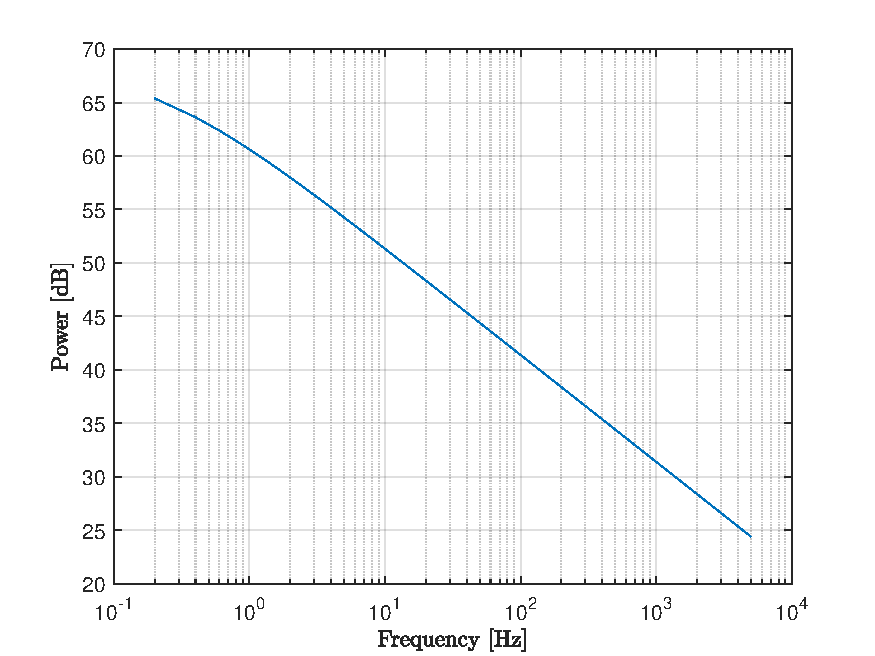
\includegraphics[width=\textwidth]{problem11_pink_noise_power_spectrum_db.pdf}
        \caption{Low Dur}
    \end{subfigure}
    \quad
    \begin{subfigure}[b]{0.31\textwidth}
        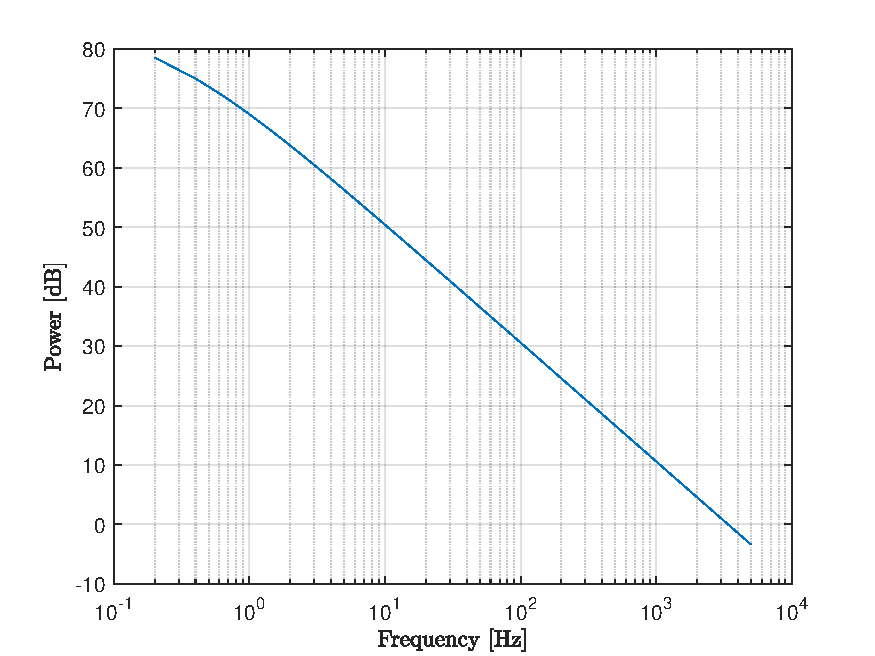
\includegraphics[width=\textwidth]{problem11_brown_noise_power_spectrum_db.pdf}
        \caption{Low Dur}
    \end{subfigure}
    \caption{Power Spectrum of Color Noise\vspace{-0.5cm}}
    \label{color_noise_freq_domain}
\end{figure}

\section{Simpler Generation of Uniform Random (White) Noise}
Done. For $U \sim \mathcal{U}(0,1)$ and $W$ to be uncorrelated uniform white noise signal in the PCM encoding, i.e. $W \in [-1,1]$, we can use the simple transform:
\[
    W = 2 U - 1
\]

Can be verified in the frequency domain. Time domain sequence given in \ref{uniform_white_noise}.

\begin{figure}[ht]
    \centering
    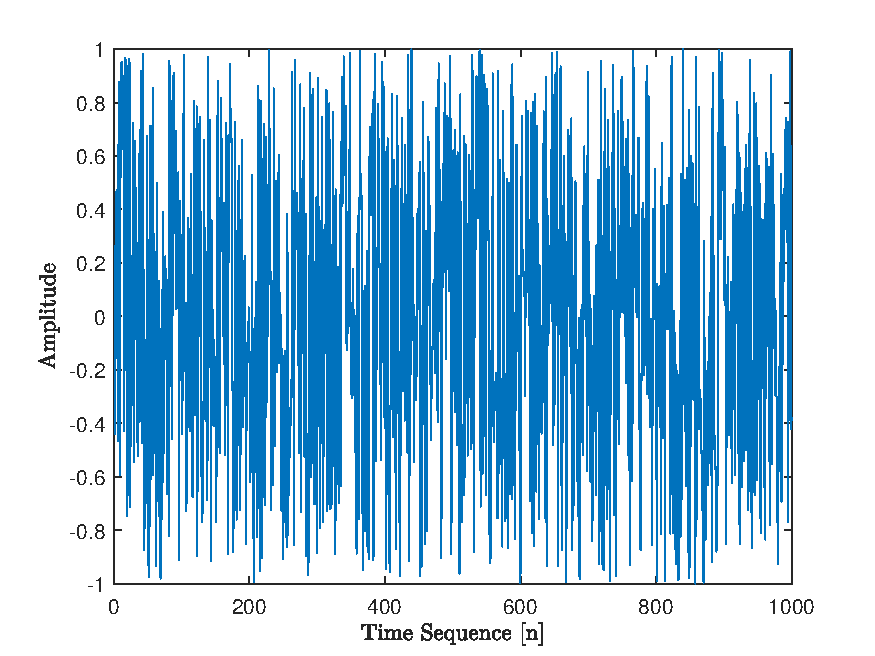
\includegraphics[width=0.5\textwidth]{problem12_uniform_white_noise_sequence.pdf}
    \caption{Uniform White Noise Sequence\vspace{-0.5cm}}
    \label{uniform_white_noise}
\end{figure}

\newpage
\clearpage
\section*{Appendix}

MATLAB code for prob 4, dialtone decode algorithm, goes here.

\begin{lstlisting}
% simple dtmf decode algorithm for a subset of tones (can be extended)
input_dtmf_tone = '';
[signal, Fs]    = audioread(input_dtmf_tone);

N   = length(signal);   % number of points in input signal and its fft
df  = Fs/N;             % frequency increment in nyquist range
fr  = -Fs/2:df:Fs/2-df; % frequency range (nyquist range)

fr_eps      = 10;         % frequency window around pure tones
dtmf_matrix = [1 2; 4 5]; % (partial) dtmf decode matrix; indexed by lower and upper band freqs
signal_fft  = fftshift(fft(signal)); % fft of the input signal

% get magnitude of each tone's contribution to the signal spectrum
m_fl1 = sum(2*abs(signal_fft(abs(fr - fl1) < fr_eps)));
m_fl2 = sum(2*abs(signal_fft(abs(fr - fl2) < fr_eps)));
m_fu1 = sum(2*abs(signal_fft(abs(fr - fu1) < fr_eps)));
m_fu2 = sum(2*abs(signal_fft(abs(fr - fu2) < fr_eps)));

% get dtmf decoding matrix indexes
[~, fl] = max([m_fl1 m_fl2]);
[~, fh] = max([m_fu1 m_fu2]);

dtmf_tone = dtmf_matrix(fl, fh); % algorithm output
\end{lstlisting}

\end{document}